\scanpage{12}
Donnée de $q$ équivaut : la donnée de
$\sigma\in
\tikz[baseline=(aut.base)]{
  \node[inner sep=0pt] (aut) {$\operatorname{Aut}^{\pm1}$};
  % Two tiny detached traces above the left of A; writing or surface marks uncertain.
  \node[anchor=south,inner sep=0pt] at ([xshift=-.12em,yshift=.12em]aut.north west)
  {\unsure{\tikz[x=1mm,y=1mm]{\fill (0,.65) circle (.12);\fill[opacity=.45] (0,0) ellipse (.10 and .16);}}};
}(\unsure{G|Z},T)$
\[
\left\{\begin{aligned}p(\sigma)&=-1\\ \sigma^2&=1\end{aligned}\right.
\]
\[
\begin{aligned}
&q_t(-1)=\sigma_t\\[.6ex]
&\sigma_{tg}=g\,\sigma_t\,g^{-1}
=g\,\underbrace{\sigma_t\,g^{-1}\,\sigma_t^{-1}}_{g}\,\sigma_t
=g^2\,\sigma_t=\sigma_t\,g^{-2}\\
&\hspace{15em}\boxed{\sigma_{tg}=g^2\sigma_t=\sigma_t g^{-2}}
\end{aligned}
\]

\uline{Corollaire} Si $n$ impair, $t\longmapsto\deleted{\unsure{q|g}}\sigma_t$ est une bijection de $T$ avec l'ens \deleted{\unsure{des}} $p^{-1}\{-1\}$; donc si on a un \unsure{pl.|pol.} à un nb impair de cotés, l'applic\textsuperscript{n} $t\longmapsto\sigma_t$ qui, à tt sommet du polygone, associe l'unique \unsure{autom} non orienté qui fixe ce sommet, est bijection.

\uline{NB} Si $n$ pair, \deleted{elle} ce n'est pas bijectif, \deleted{\unsure{mais}} \deleted{\unsure{pour tt}} ses fibres sont vides ou de cardinal 2\ldots

% slanted left margin note; the line nodes preserve the cramped oblique geometry.
\reversemarginpar
\margin{\vspace*{-2.7\baselineskip}\hspace*{-1.05cm}%
\begin{tikzpicture}[x=.007cm,y=.007cm,baseline=(0,0)]
  \node[anchor=base west,rotate=34,inner sep=0pt] at (31,-115) {$\{u,\bar u\}\subset Z$};
  \node[anchor=base west,rotate=34,inner sep=0pt] at (15,-183) {gén. opposés d'ordre};
  \node[anchor=base west,rotate=34,inner sep=0pt] at (10,-239) {$n=2m$, alors};
  \node[anchor=base west,rotate=34,inner sep=0pt] at (30,-291) {$u^m=\bar u^m=s$, \uline{unique}};
  \node[anchor=base west,rotate=34,inner sep=0pt] at (23,-348) {\uline{\unsure{élémt|élément} d'ordre} 2 de $Z$};
  \node[anchor=base west,rotate=34,inner sep=0pt] at (25,-412) {appelé symétrie};
  \node[anchor=base west,rotate=34,inner sep=0pt] at (25,-465) {Mon $\sigma_t=\sigma_{t'}$};
  \node[anchor=base west,rotate=34,inner sep=0pt] at (35,-520) {\unsure{sss|ssi} $t,t'$ sont \unsure{conjugués}};
  \node[anchor=base west,rotate=34,inner sep=0pt] at (43,-565) {mod $\{1,s\}$};
  % The separate upright and the thinner curved boundary are not mathematical arrows.
  \draw[line width=.45pt] (313,-5) -- (319,-179);
  \draw[line width=.28pt] (285,-73) -- (307,-154)
    .. controls (337,-187) and (393,-193) .. (427,-193)
    .. controls (377,-221) and (337,-255) .. (335,-281)
    .. controls (342,-359) and (375,-401) .. (334,-476)
    .. controls (291,-536) and (222,-603) .. (152,-665);
\end{tikzpicture}}
\normalmarginpar

\uline{Sommet} \uline{opposé}, symétrie canonique

\uline{Parenthèse}\qquad Produit fibré d'ens

\diagram{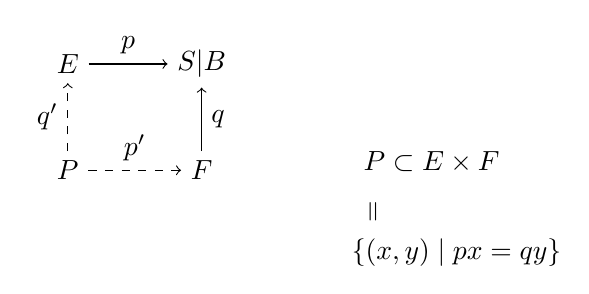
\begin{tikzpicture}[x=1cm,y=1cm]
  \node (E) at (0,0) {$E$};
  \node (S) at (1.7,0) {$\unsure{S|B}$};
  \node (P) at (0,-1.35) {$P$};
  \node (F) at (1.7,-1.35) {$F$};
  \draw[->] (E) -- node[above] {$p$} (S);
  \draw[->,dashed] (P) -- node[left] {$q'$} (E);
  \draw[->,dashed] (P) -- node[above] {$p'$} (F);
  \draw[->] (F) -- node[right] {$q$} (S);
  % The first set-display line starts level with the lower row of the square.
  \node[anchor=base west,inner sep=0pt] at (3.75,-1.35) {$P\subset E\times F$};
  \node[inner sep=0pt] at (3.9,-1.88) {\rotatebox{90}{$=$}};
  \node[anchor=base west,inner sep=0pt] at (3.60,-2.48) {$\{(x,y)\mid px=qy\}$};
\end{tikzpicture}}
% Detached pair of points to the far right of the set display; no punctuation function assigned.
\margin{\raisebox{1.2em}{\unsure{\tikz[x=1mm,y=1mm]{\fill (.45,.8) circle (.12);\fill (0,0) circle (.12);}}}}

\unsure{$s$}

Solution d'un Pb universel dans la cat. des ens :

Si $E,F,S$ des \unsure{groupes|grpes}, $p,q$ hom de \unsure{grpe|groupe}, alors $P$ un \unsure{grpe|groupe} (et solution du pb univ. analogue \unsure{ds|dans} cat. des \unsure{grpes|groupes})
\[
\operatorname{Ker}p\sim\operatorname{Ker}p',\quad
\operatorname{Ker}q\sim\operatorname{Ker}q'
\]

Si $p$\tikz[baseline=(surj.base)]{
  \node[anchor=base west,inner sep=0pt] (surj) at (0,0) {surjectif};
  \node[anchor=base west,inner sep=0pt] at (-.05, .39) {\inserted{$:E\mathbin{\text{---}}S$}};
  \draw[line width=.3pt] (.02,.12) .. controls (.24,.32) and (.65,.30) .. (.94,.40);
}\ bijectif) alors $P\mathbin{\text{---}}F$ surjectif (bijectif).

[Langage des
\tikz[baseline=(old.base)]{
  \node[anchor=base,inner sep=0pt] (old) at (0,0) {\deleted{\unsure{diagrammes}}};
  \node[anchor=base,inner sep=0pt] at (.12,.38) {\inserted{carrés}};
}
cartésiens]

Image inverse d'ex. de \unsure{groupe|groupes|grpe}
% archive sheet number: 11
